\chapter{Introduction}

In this chapter, we introduce the motivation to build a highly available web service in rural area. We illustrate the result of observation and identify the key problems.

In chapter \ref{sync}, we start by formulating the problem into a multi-master system, and then investigate several available technologies that address this challenge. We examine them against our unique requirement and select one as our basis. We then propose and explain our approach on top of it.

In chapter \ref{benchmark}, we illustrate the idea of using ARM-based hardware to achieve low-power consumption web service. To study the capacity of hardware, we benchmark the performance of each components of web service on different platform. According to the result, we propose a cluster than can be easily scaled out to serve more users.

In chapter \ref{conclusion}, we draw our conclusion and shed light on future work.
\section{Background}
Affordable, yet stable web services are highly desired in rural area, as a mean to alleviate digital divide and improve life quality. When it comes to under-developed regions in Africa, requirements and conditions need to be carefully assessed and analyzed, for that challenges could be unique and dramatically different than metropolitan.

\section{E-learning for Open University of Tanzania} \label{out_intro}
%database-driven and static
Open University of Tanzania (OUT) \cite{out} is the first university of East Africa Region to provide open and distance learning programmes. To distribute course content through the whole country, Moodle has been chosen as underlying digital resource management platform. Moodle\cite{moodle} is an open-source industrial-level online learning platform and resource management system. As a typical data-driven web service, Moodle runs over an underlying database and assemble its webpages on-the-fly based on user requests. It is written in PHP and heavily tested against Apache, Nginx and MySQL. At present, the platform is running as a standalone web service in a central server and mainly serve static content such as PDF, Text and Slides. Although OUT has the vision to introduce multi-media materials to enhance education quality. OUT also establishes learning centers in major cities and towns all over the whole country and is ambitious to extend to a larger scale. An emerging obstacle is to provide services in remote areas with poor network connection and bandwidth.

\section{Problem Identification}
%Objectives to achieve in this projects.
%Goals
As part of the project, we investigated local conditions and needs within the scale of Serengeti Broadband Network, especially in areas with evident demands of services and lack of infrastructures. And we were able to identify following challenges:

\subsection{Power Outages}
%ellaborate this paragraph
Power grid in rural areas of Tanzania is so unreliable that UPS for critical device is almost a must. While people are gradually adapting to mobile platforms, such as smart phones and tablets, backbone infrastructures are also required to be more persistent. Equipments powered up by solar and battery are highly desired due to cost-efficiency. Although power consumption need to be optimized in this circumstance in order to prolong battery life and improve reliability.

\subsection{Poor network quality and frequent failure}
Although local network is operated by ICT4RD project and can be fairly reliable, uplink is still depending on national-wide ISP and is somewhat unpredictable according to our observation. Network failure could occur anytime and can last for random period (several minutes to several days). Those web services that depend on a central server are apparently not accessible during the failure. On the other hand, the uplink can be very narrow due to poor infrastructure and limited budget. It could be difficult to squeeze multimedia services into such bandwidth.

To better illustrate this problem, suppose a typical setting in Figure \ref{rural_lan}. Major backbone components in this LAN are interconnected through fiber-optical lines, and network is distributed to users through WiFi or Ethernet. The LAN is linked to the Internet through ISP distribution link and central server resides on the otherside of the Internet.

\begin{figure}[htbp]
\centering
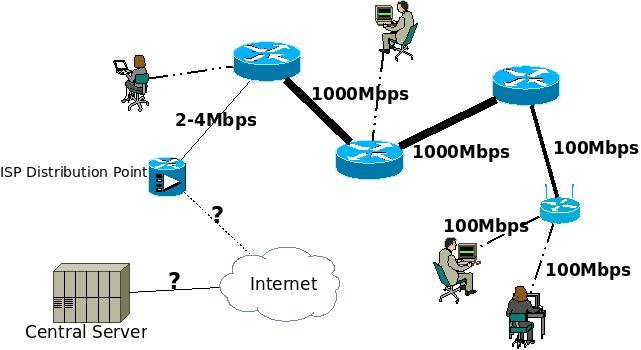
\includegraphics[width=0.8\textwidth]{../images/brief_diagram_of_sbn_network.jpeg}
\caption{A Typical Setting of Rural Local Access Network (LAN)}
\label{rural_lan}
\end{figure}

Due to limited budget and ISP capacity, the upper link is equipped with an average bandwidth of 2~4Mbps which is shared among all users in LAN. While a minimum bandwidth of 1.5Mbps is recommended for video streaming, it is difficult for users to get decent service from central server.
To worsen the situation, the upper link is somewhat unpreditable, which leads to the isolation of LAN, as shown in \ref{uplink_break}.

\begin{figure}[htbp]
\centering
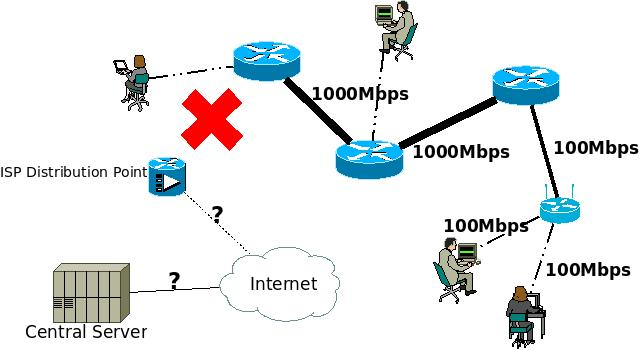
\includegraphics[width=0.8\textwidth]{../images/brief_diagram_of_sbn_network_upper_broken.jpeg}
\caption{Uplink Failure leads to the isolation of LAN}
\label{uplink_break}
\end{figure}

On the other hand, components in the LAN can also break down which leads to network separation, see Figure \ref{nata_break}. In the first case, multi-media content can hardly reach end users. And in other two cases, users cannot get service at all.

\begin{figure}[htbp]
\centering
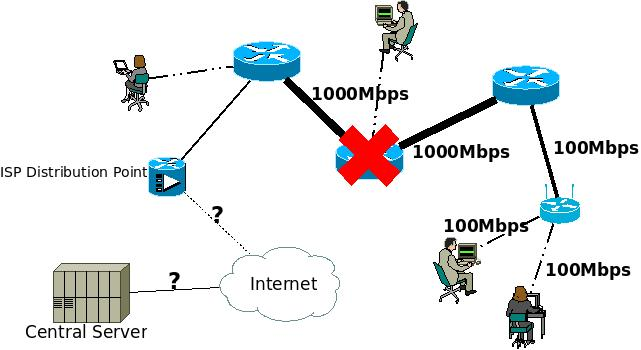
\includegraphics[width=0.8\textwidth]{../images/brief_diagram_of_sbn_network_nata_broken.jpeg}
\caption{Network Separation due to Component Failure}
\label{nata_break}
\end{figure}

\subsection{Limited budget}
Cost is an essential factor during rural ICT development. Given relatively smaller user base and weaker demand, equipments need to be chosen wisely. Although future maintainence and development also need to be considered.